% !TEX root = ../main.tex

\chapter{Experiments}
\label{ch:experiments}

\section{Research Questions}
To analyze and compare the different models, I formulated the following research questions:
\begin{enumerate}
  \item How do function approximators other than neural networks compare with the latter?
  \item Bias
\end{enumerate}

\section{Experiments}
To investigate and answer the formulated research questions, I conducted the following experiments:
\begin{enumerate}
  \item Similar to \citet{oller_analyzing_2020}, I used RWG to draw the weights of the models and tested the performance on a Classic Control environment from OpenAI Gym.
  \item Second experiment
\end{enumerate}
In the first experiment, analogous to \citet{oller_analyzing_2020}, there is no learning involved. For their paper, they were interested in the complexity of the environment, whereas I aim to find out more about the nature of the models. I selected a few candidates for the models, which are described in Section~\ref{ssec:models} and used them for a series of experiments. I used the same procedure for all models, which allows me to compare them with one another. For the experiments, first, I initialized the environment. I used the \verb|CartPole| and \verb|Acrobot| environment for these experiments. These environments are fairly easy to solve, as explained in Section~\ref{ssec:benchmarks}. Therefore, we expect some controllers to solve the task even without any training. Second, I initialized the respective model. Then, I drew the model weights from the standard normal distribution $\mathcal{N}(0,1)$. Each of these instances of the model represents a sample. In total, I used $10'000$ samples ($N_{samples}$). Finally, I ran 20 episodes ($N_{episodes}$) with each sample for an environment and stored the respective score as an entry of the score tensor $S$. Algorithm~\ref{alg:model-evaluation} shows an overview of the described procedure.
\begin{algorithm}
\caption{First experiment with RWG}
\begin{algorithmic}[1]
\State Initialize environment
\State Initialize model
\State Create array $S$ of size $N_{samples} \times N_{episodes}$
\For{$n = 1,2,...,N_{samples}$}
    \State Sample model weights randomly from $\mathcal{N}(0,1)$
    \For{$e=1,2,...,N_{episodes}$}
      \State Reset the environment
      \State Run episode with model
      \State Store accured episode reward in $S_{n,e}$
    \EndFor
\EndFor
\end{algorithmic}
\label{alg:model-evaluation}
\end{algorithm}

\subsection{OpenAI Gym Environments}
\begin{itemize}
  \item CartPole
  \item Acrobot
\end{itemize}

\todo[inline]{Explain used environments}

\subsection{Models}
\label{ssec:models}
For the polynomial model, I used two architectures $P_1$ and $P_2$. The first model $P_1$ consists of one polynomial for each possible action in a discrete action space. The input of the model is the observation from the environment. The dimension of the weight vectors is according to the dimension of the input vector. For the environment \verb|CartPole| with the discrete action space $\{0, 1\}$ and observation $x = [x_0, x_1, x_2, x_3]^T$, this means that $P_1$ consists of two polynomials:
\[
  p_0(x) = \Sigma_{i=0}^{n} w_i^T (x_k^i)_{k \in I} \in \mathbb{R}, \ \ \ \ \ \ \ \ \ \ w_i \in \mathbb{R}^4, \ \ I = \{0, 1, 2, 3\}
\]
\[
  p_1(x) = \Sigma_{j=0}^{n} w_j^T (x_k^j)_{k \in I} \in \mathbb{R}, \ \ \ \ \ \ \ \ \ \ w_j \in \mathbb{R}^4, \ \ I = \{0, 1, 2, 3\}
\]
In the formulas, $n$ denotes the degree of the polynomial. In the experiments, I tested polynomials with degrees 1, 2, and 3. The output of the polynomials has no reasonable upper and lower limit, as illustrated in Figure~\ref{fig:bounds}. That makes it harder to interpret the results reasonably.
\begin{figure}[ht]
\centering
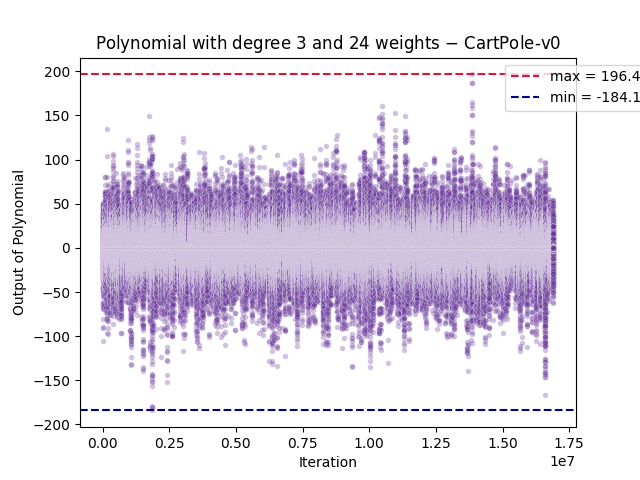
\includegraphics[width=0.6\textwidth]{PolynomialNN_degree_3_bounds}
\caption[Upper and lower bound]{
  \textbf{Upper and lower bound.}
  The figure shows each output of the polynomial functions described above. As we can see, the functions are not well bound, and there are quite a few outliers. That makes it hard to interpret the output sensibly.
}
\label{fig:bounds}
\end{figure}
So, I scaled the outputs with a sigmoid function. A sigmoid function is a mathematical function that maps an arbitrary input space into an output space with a small range, for example, 0 and 1. The function has a characteristic S-shaped curve. We can interpret the output space of the sigmoid function as a probability. In this case, we search for the probability that a specific action is the reasonable one given an observation $x$. Thus, for our example with the \verb|CartPole| environment, we can interpret $sig(p_0)$ as the probability that action 0 is the correct one and $sig(p_1)$ as the probability that action 1 is the correct one. Putting this thought into a formula for $P_1$ and the \verb|CartPole| environment, we get:
\[
  P_1(x) =
  \begin{cases}1~&{\text{ if }}~sig(p_1(x)) > sig(p_0(x))~,\\0~&~\text{otherwise}~.\end{cases}
\]
For the sigmoid function, I used the logistic sigmoid function. The formula and a plot of the function are shown in Figure~\ref{fig:sigmoid}.

\begin{figure}[ht]
\centering
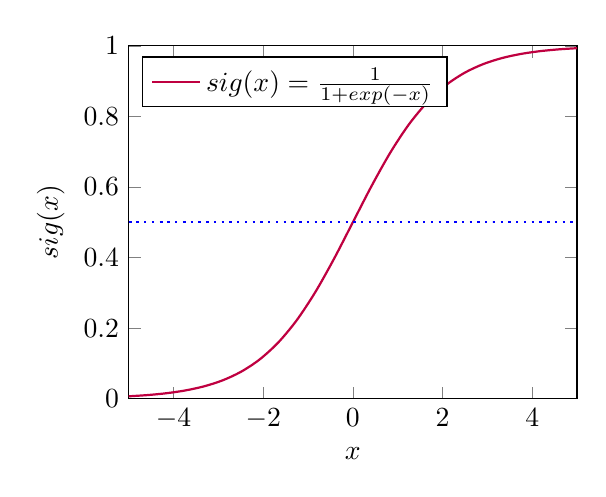
\begin{tikzpicture}
\begin{axis}[
      xmin = -5, xmax = 5,
      ymin = 0, ymax = 1,
      legend cell align = {left},
      legend pos = north west,
      width = 0.6\textwidth,
      height = 0.5\textwidth,
      xlabel = \(x\),
      ylabel = {\(sig(x)\)}
    ]
    \addplot[
        smooth,
        thick,
        purple
    ] {1 / (1 + exp(-x))};
    \addlegendentry{
    $sig(x) = \frac{1}{1 + exp(-x)}$
    }
    \addplot[
        smooth,
        thick,
        blue,
        dotted
    ] {0.5};
\end{axis}
\end{tikzpicture}
\caption[Sigmoid function]{
  \textbf{Sigmoid function.}
  The figure shows a plot of the logistic sigmoid function. The function maps an arbitrary input space into the range between 0 and 1. The output of the function can be interpreted as a probability. It is useful to scale data into a meaningful value.
}
\label{fig:sigmoid}
\end{figure}


The second model $P_2$ is constructed similarly to $P_1$, but it only consists of one polynomial instead of one for each possible action. For the \verb|CartPole| environment, this means $P_2$ consists of:
\[
  p(x) = \Sigma_{i=0}^{n} w_i^T (x_k^i)_{k \in I} \in \mathbb{R}, \ \ \ \ \ \ \ \ \ \ w_i \in \mathbb{R}^4, \ \ I = \{0, 1, 2, 3\}
\]
Analogous to $P_1$, I tested the polynomial $p(x)$ with degree 1, 2, and 3. So, $n \in \{1, 2, 3\}$. In addition, I again used the logistic sigmoid function to scale the output of the polynomial. However, the output of the $P_2$ is determined by a fixed threshold instead of comparing multiple polynomials. Putting this into a formula for the \verb|CartPole| environment, we get:
\[
  P_2(x) =
  \begin{cases}1~&{\text{ if }}~sig(p(x))>0.5~,\\0~&~\text{otherwise}~.\end{cases}
\]


\section{Results}
\subsection{Experiment 1}
Figure~\ref{fig:experiment_1_polynomial} shows the results of the first experiment for the two architectures of the polynomial model $P_1$ and $P_2$. I visualized the results of each model working with a bias in row (a) and without bias in row (b). The structure of the plots is identical for better comparison. The samples are ranked according to their mean score and aligned on the $x-$axis according to their rank. The scatter plots show all scores of the samples, whereas the lineplot illustrates the mean of each sample over all episodes.
Subfigure~\ref{fig:results_p1} shows the results of the polynomial model $P_1$ and Subfigure~\ref{fig:results_p2} shows the results of the polynomial model $P_2$.
\begin{figure}[!ht]
\begin{subfigure}{\textwidth}
\begin{figrow}
\item \label{row:P1_with_bias} \raisebox{-0.5\height}{
\includegraphics[width=.3\linewidth]{experiment_1/with_bias/PolynomialNN_degree_1_scatter_score.png}
\includegraphics[width=.3\linewidth]{experiment_1/with_bias/PolynomialNN_degree_2_scatter_score.png}
\includegraphics[width=.3\linewidth]{experiment_1/with_bias/PolynomialNN_degree_3_scatter_score.png}}
\item \label{row:P1_without_bias}  \raisebox{-0.5\height}{
\includegraphics[width=.3\linewidth]{experiment_1/without_bias/PolynomialNN_degree_1_scatter_score.png}
\includegraphics[width=.3\linewidth]{experiment_1/without_bias/PolynomialNN_degree_2_scatter_score.png}
\includegraphics[width=.3\linewidth]{experiment_1/without_bias/PolynomialNN_degree_3_scatter_score.png}}
\end{figrow}
\vspace*{-5mm}
\caption{Results of $P_1$ with bias (a) and without bias (b)}
\label{fig:results_p1}
\end{subfigure}
\begin{subfigure}{\textwidth}
\begin{figrow}
\item \label{row:P2_with_bias} \raisebox{-0.5\height}{
\includegraphics[width=.3\linewidth]{experiment_1/with_bias/Polynomial_degree_1_scatter_score.png}
\includegraphics[width=.3\linewidth]{experiment_1/with_bias/Polynomial_degree_2_scatter_score.png}
\includegraphics[width=.3\linewidth]{experiment_1/with_bias/Polynomial_degree_3_scatter_score.png}}
\item \label{row:P2_without_bias}  \raisebox{-0.5\height}{
\includegraphics[width=.3\linewidth]{experiment_1/without_bias/Polynomial_degree_1_scatter_score.png}
\includegraphics[width=.3\linewidth]{experiment_1/without_bias/Polynomial_degree_2_scatter_score.png}
\includegraphics[width=.3\linewidth]{experiment_1/without_bias/Polynomial_degree_3_scatter_score.png}}
\end{figrow}
\vspace*{-5mm}
\caption{Results of $P_2$ with bias (a) and without bias (b)}
\label{fig:results_p2}
\end{subfigure}
\caption[Results of experiment 1]{
  \textbf{Results of experiment 1.}
   The figures show the results of the first experiment with the two polynomial models. On the $x-$axis, we have the rank of each sample. On the $y-$axis, we have the scores of all samples and the mean as a lineplot. Each subplot shows the performance of the model with bias in row (a) and without bias in row (b). As we can see, both models perform equally good or bad. However, there is a huge difference in performance whether we are working with or without bias. In addition, we can see a difference in the slope of the mean values between polynomials with degree 1 and one with a higher degree.
}
\label{fig:experiment_1_polynomial}
\end{figure}
As we can see in the images, the plots of the two models almost look identical. Both models performed equally good or bad despite their different architecture and the different number of weights. Because of this similarity, I will not go into each model independently but instead discuss further results for both of them.

Looking at the linear model without bias, we can see a striking resemblance to the performance of the neural network previously shown in Section~\ref{ssec:benchmarks}. Looking further at the linear model, we can see that the curve of the mean score stays low until around $5'000$ but then goes up relatively steeply. That means that the linear model fails around 50\% miserably. However, after that, we have a high probability to achieve a good score or even solve the task entirely during multiple episodes. There are also quite a few samples that could solve the task each time, indicated by the short straight black line at the top of the plot. Looking at the polynomials with degree 2, we can see that the scores increase already at around $2'000$, but the slope is less steep than for the linear model. In addition, there are fewer samples that could solve the task for each episode than there are for the linear model. If we look at the results of the polynomials with degree three, we can see that there is only a small boost compared to the polynomials of degree 2. The scores are overall slightly higher, but the slope is very similar to before. There is only a little difference between the two models even though the weights are doubled for $P_1$ and a half more for $P_2$. The large difference lies between the polynomials with degree 1 and polynomials with degree 2, respectively, degree 3. It seems that the complexity of the model depends more on the architecture of the model than on the number of weights.

In conclusion, with the linear model, we have a $50 \%$ chance of failing but the probability of actually solving the task for all episodes is higher than for the polynomials with a higher degree. That means that with the linear model, we have a larger fraction of samples that can solve the environment independent of the initialization conditions. At first glance, we could assume that this is an important aspect for such a model and choose the polynomial with degree 1 over one with a higher degree. However, we should remind ourselves that these experiments are rather unusual for an application since there is no learning involved and the number of samples is huge. In a common application, we would use some kind of training and want the model to sequentially improve its performance. Considering this aspect, when using a learning algorithm, we would not prefer the polynomials with degree 1 as we might get stuck in a fitness plateau when the algorithm has no method of dealing with this behavior.

Another observation we can make from Figure~\ref{fig:experiment_1_polynomial} is that the bias influences the performance of the model significantly. We already saw this behavior with the neural network in Section~\ref{ssec:benchmarks}. Thus, the influence of the bias is not specific to neural networks but seems to be more of a general factor.

\todo[inline]{Change title of plots: , instead of with, $P_1 / P_2$ instead of Polynomial}
